%%%% Better Poster latex template example v1.0 (2019/04/04)
%%%% GNU General Public License v3.0
%%%% Rafael Bailo
%%%% https://github.com/rafaelbailo/betterposter-latex-template
%%%% 
%%%% Original design from Mike Morrison
%%%% https://twitter.com/mikemorrison

\documentclass[a0paper,fleqn]{src/betterposter}

\begin{document}	
\betterposter{
%%%%%%%% MAIN COLUMN

\maincolumn{
%%%% Main space

\textbf{From code to deployment}\\
\fontsize{75}{77}\selectfont % Set the font size to 12pt with a baseline skip of 14pt

Pull-request workflow\\[1.5cm]
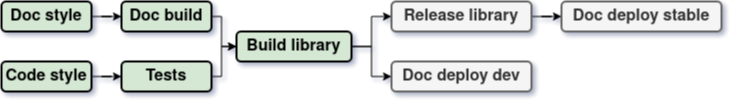
\includegraphics[width=\textwidth]{img/ci_cd/ci_cd_pr}\\

Main branch workflow\\[1.5cm]
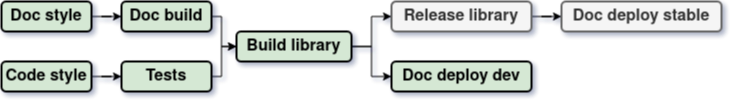
\includegraphics[width=\textwidth]{img/ci_cd/ci_cd_main}\\

Release workflow\\[1.5cm]
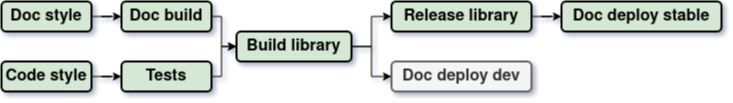
\includegraphics[width=\textwidth]{img/ci_cd/ci_cd_release}\\

\fontsize{85}{87}\selectfont
Use ansys/actions@v4\\[1cm]

\vspace{-18cm}

}{
%%%% Bottom space

%% QR code
\qrcode{img/ci_cd/qrcode.png}{img/general/smartphoneBlack}{
\textbf{Visit https:\slash \slash actions.docs.ansys.com for more information}
}
% Smartphone icon
% Author: Freepik
% Retrieved from: https://www.flaticon.com/free-icon/smartphone_65680

%% Compact QR code (comment the previous command and uncomment this one to switch)
%\compactqrcode{img/example/qrcode}{
%\textbf{Take a picture} to
%\\download the full paper
%}

}

}{
%%%%%%%% LEFT COLUMN

\title{CI\slash CD pipelines for scientists}
\author{Jorge Martinez}
\institution{Ansys}

\section{
\includegraphics[height=\fontcharht\font`\S]{img/general/slash.png} Introduction}
Continuous integration (CI) and continuous delivery (CD) is used for empowering
software development through automated integration and deployment,
revolutionizing efficiency and reliability in the software delivery lifecycle.

\section{
\includegraphics[height=\fontcharht\font`\S]{img/general/slash.png} Code style}
Enforcing consistency and code quality through automated analysis, ensuring
clean and maintainable software development practices.

\section{
\includegraphics[height=\fontcharht\font`\S]{img/general/slash.png} Doc style}
Elevating documentation quality through automated analysis, fostering clear and
consistent communication for comprehensive software documentation.

\section{
\includegraphics[height=\fontcharht\font`\S]{img/general/slash.png} Doc build}
Streamlining the creation of documentation through automated processes, enabling
efficient and accurate documentation generation for seamless project
collaboration.

\section{
\includegraphics[height=\fontcharht\font`\S]{img/general/slash.png} Tests}
Enhancing software quality through systematic and efficient test automation,
ensuring robustness, reliability and code coverage in the development process.


%% This fills the space between the content and the logo
%\vfill

%% Institution logo
%
\includegraphics[width=\textwidth]{img/general/pyansys_dark}\\

}{
%%%%%%%% RIGHT COLUMN

\section{
\includegraphics[height=\fontcharht\font`\S]{img/general/slash.png} Build library}
Leveraging pre-built components and artifacts to expedite software development,
enhancing efficiency and scalability in the creation of complex applications.

\section{
\includegraphics[height=\fontcharht\font`\S]{img/general/slash.png} Release}
Leveraging pre-built components and artifacts to expedite software development,
enhancing efficiency and scalability in the creation of complex applications.

\section{
\includegraphics[height=\fontcharht\font`\S]{img/general/slash.png} Doc deploy}
Streamlining the distribution and accessibility of developer and user
documentation. Empowering teams and customers with up-to-date resources for
seamless collaboration and knowledge sharing.

\vfil


\includegraphics[width=\textwidth]{img/general/pyansys_dark}\\
%\section{
\includegraphics[height=\fontcharht\font`\S]{img/general/slash.png} What is PyAnsys?}
The PyAnsys project is a collection of Python packages that enable the use of Ansys products through Python.
\\
\newline
\textbf{Any doubts?} \\Contact us at pyansys.core@ansys.com!
\\
\newline

\qrcode{img/general/pyansys_qrcode.png}{img/general/smartphoneBlack}{
\textbf{\huge{Check our docs for more\\information on PyAnsys!\\https:\slash \slash docs.pyansys.com }}
}
}
\end{document}
